\section{Introduction}

EchoGAE~\supercite{Alatawi2023EchoGAE} trains a two-layer graph autoencoder on a Twitter retweet graph, detects communities, and returns an Echo Chamber Score (ECS) per topic. A larger ECS is read as evidence that the conversation on that topic exhibits stronger echo-chamber structure. The original paper reports ECS values of $0.714$, $0.626$, $0.485$, and $0.465$ on gun control, abortion, Super Bowl, and SXSW, and argues that the polarising pair (gun control, abortion) scores higher than the non-polarising pair (Super Bowl, SXSW).

This article reports the outcome of a reproduction of those four values using the released source, the released raw inputs, regenerated text features, and the released computation. Three findings organise the report. First, the released notebook stores ECS values of $0.628$, $0.622$, $0.562$, and $0.465$. These differ from the paper's table on three of the four topics and, as far as we have found, have not been discussed in the subsequent literature. Second, the notebook implements an average of per-user scores, while the paper's Equation~4 specifies an average of per-community scores. On graphs with unequal community sizes these give different quantities. Third, on SXSW at the released seed and architecture, ten fits give a user-average score of $0.467 \pm 0.007$, within one standard deviation of the paper's $0.465$; the same fits averaged by community give $0.655 \pm 0.006$. The reproduction therefore succeeds under the released code's averaging rule, and documents a definitional ambiguity between the paper's equation and the released implementation.

Averaging per-point scores at the item level or at the cluster level is a long-standing distinction in cluster validation. The silhouette coefficient~\supercite{Rousseeuw1987} is widely reported as either a per-point mean or a per-cluster mean, under identical names, and the two differ whenever cluster sizes are unequal. Discussions of micro-versus-macro averaging in classification~\supercite{YangLiu1999} and in information retrieval~\supercite{Manning2008IR} raise the same point: both averages are defined, both are useful, and neither can substitute for the other without a comment on what the reported number counts. ECS inherits that structure through its silhouette-style construction. The ambiguity we document is an instance of this familiar measurement choice, and our reproduction protocol separates it from other pipeline differences.

The reproduction is classified Rp (reproduction) in the ReScience sense~\supercite{RougierReScience2017}: same code, same raw inputs, with only the minimal patch needed to parameterise the fitting seed. A structural experiment retrains the released model on rewired graphs; we report it as a sensitivity check, not as a reproduction of the original paper's figures.

\section{The score and its two aggregations}
\label{sec:score}

Let $C(v)$ denote the community of user $v$, and let $d(u,v)$ be the Euclidean distance between the fitted representations of two users. For every user $v$, the released code computes
\[
a_v=\frac{1}{|C(v)|}\sum_{u\in C(v)}d(u,v), \qquad
b_v=\min_{C\ne C(v)}\frac{1}{|C|}\sum_{u\in C}d(u,v),
\]
and, when another community exists and $\max(a_v,b_v)>0$,
\[
s_v=\frac{b_v-a_v+\max(a_v,b_v)}{2\max(a_v,b_v)}.
\]
Thus $s_v\in[0,1]$, with $s_v=\tfrac{1}{2}$ when $a_v=b_v>0$. For $n$ users partitioned into $K$ communities of sizes $n_k$ with within-community mean score $\bar s_k$, the two graph-level aggregations are
\[
S_{\mathrm{user}}=\sum_{k=1}^K \frac{n_k}{n}\,\bar s_k, \qquad
S_{\mathrm{community}}=\frac{1}{K}\sum_{k=1}^K \bar s_k,
\]
with difference
\[
S_{\mathrm{community}}-S_{\mathrm{user}}=\sum_{k=1}^K\!\Big(\tfrac{1}{K}-\tfrac{n_k}{n}\Big)\bar s_k.
\]
The sign and magnitude of the difference depend on how community size and per-community mean covary across the partition.

The paper's Equation~4 is written as $S_{\mathrm{community}}$ and attributed as a sum over communities; the released notebook (\texttt{ECS.evaluate}) computes $S_{\mathrm{user}}$. Both appear in the literature under the same name.

Two arithmetic observations from the original paper are consistent with its reported values coming from $S_{\mathrm{user}}$. On gun control the paper reports per-community scores $0.739$ and $0.676$ with community sizes $3{,}984$ and $2{,}582$; the unweighted mean is $0.7075$, the size-weighted mean is $0.7142$, and the reported graph score is $0.714$. Accepting the rounding on the per-community scores, the size-weighted mean matches the reported value and the unweighted mean does not. The remaining mismatches between the paper's table and the notebook's stored values are discussed in Section~\ref{sec:residuals}.

\section{Reproduction protocol}
\label{sec:protocol}

We fix the source and the raw inputs, regenerate text features, and separate fitting from community detection.

\subsection{Pinned source and inputs}

The EchoGAE release is pinned to commit \texttt{0626330}. Our notebook, loader, score implementation, and tweet preprocessor match that snapshot byte for byte. All twelve shipped raw graph, tweet, and label files match the release's Git blob hashes. A seed-parameterisation patch exposes the fitting seed as an argument to the model function and is applied as a separate patch on top of the unchanged release source.

The notebook explicitly sets the autoencoder's hidden and output widths to $20$ and $10$; the Python function, if called without those arguments, defaults to $100$ and $50$. We follow the notebook's explicit settings. A control run under the defaults is reported in Section~\ref{sec:residuals}.

The loader intersects each graph with users having text features and retains the largest connected component. On the four topics the processed graphs contain, in (users, edges), $(6{,}566, 14{,}322)$ on gun control, $(5{,}087, 10{,}572)$ on abortion, $(5{,}460, 8{,}732)$ on Super Bowl, and $(2{,}436, 5{,}325)$ on SXSW, matching the published Table~I.

\subsection{Regenerated text features}

The release ships cached Sentence-BERT embeddings. Their provenance (model revision, preprocessing, encoded tweet count) is not documented. We regenerate the features from the shipped tweets using Sentence-BERT \texttt{all-MiniLM-L6-v2} revision \texttt{1110a243}, averaging within users. The regenerated feature file hashes and the counts of encoded tweets are recorded in the artifact. The cached embeddings are retained only for a diagnostic comparison; all reported numbers use the regenerated features.

Feeding the regenerated features through the unmodified upstream loader reproduces the graph edges, the ordered feature matrix, and the seed-$42$ Louvain partitions exactly. The score computation is checked against the upstream implementation, including its convention of including each vertex's zero within-community self-distance in $a_v$.

\subsection{Crossed seed design}

Fitting the autoencoder is independent of the Louvain partition used for scoring. We cross ten Louvain seeds ($42$--$51$, resolution $0.05$) with ten fitting seeds ($42$--$51$). Each of the ten fits produces one embedding per topic; each of the ten partitions produces one community assignment per topic; both graph-level averages are computed on every combination. The notebook's own configuration corresponds to the cell at Louvain seed $42$, fitting seed $42$.

An ECS that requires a nearest-other community is undefined when the detected partition has exactly one non-singleton community. A zero denominator in $\max(a_v,b_v)$ also leaves $s_v$ undefined. We record these cases explicitly rather than inserting a value. Abortion has one partition seed that returns a single non-singleton community, affecting $10$ of the $100$ seed pairs.

\subsection{Environment}

Current executions use Python 3.13.2 on macOS 26.5.2, NetworkX 3.6.1, Torch 2.12.0, PyTorch Geometric 2.8.0, NumPy 2.3.2, scikit-learn 1.8.0, and Sentence Transformers 5.1.0. Fitting uses the CPU with two Torch threads; feature encoding uses the MPS backend. The release's \texttt{environment.yml} pins NetworkX $3.1$. A separate check repeats the ten Louvain partitions under NetworkX $3.1$ on the same fixed representations; they match the NetworkX $3.6.1$ partitions exactly.

A locked environment is then rebuilt from scratch, and one full $300$-epoch SXSW reference fit at seed $42$ is run in it. The reference fit matches the primary SXSW seed-$42$ representations exactly, as does an unmodified-model control under matched random states.

\section{Results}
\label{sec:results}

\subsection{Reproduction}

Table~\ref{tab:repro} reports both averages on all four topics across ten fits at the reference partition. The paired difference in the final column uses the same fitted representations under both rules; its only source is the weighting.

\begin{table}[h!]
\centering\small
\begin{tabular}{lrrrrr}
\hline\noalign{\smallskip}
Topic & Paper & Notebook & User avg.\ & Community avg.\ & Difference \\
\noalign{\smallskip}\hline\noalign{\smallskip}
Gun control & $0.714$ & $0.628$ & $0.657\pm 0.028$ & $0.656\pm 0.027$ & $-0.001$ \\
Abortion    & $0.626$ & $0.622$ & $0.619\pm 0.017$ & $0.644\pm 0.017$ & $+0.026$ \\
Super Bowl  & $0.485$ & $0.562$ & $0.545\pm 0.011$ & $0.574\pm 0.024$ & $+0.029$ \\
SXSW        & $0.465$ & $0.465$ & $0.467\pm 0.007$ & $0.655\pm 0.006$ & $+0.187$ \\
\noalign{\smallskip}\hline
\end{tabular}
\caption{Reproduction. ``Paper'' is the value reported in Alatawi et al.\ (2023), Table~II. ``Notebook'' is the value stored in the released notebook output (cell at seed $42$). ``User avg.''\ and ``Community avg.''\ are the means $\pm$ standard deviations over ten fitting seeds at the reference partition. ``Difference'' is community minus user averaging, averaged across the same ten pairs.}
\label{tab:repro}
\end{table}

Under $S_{\mathrm{user}}$, SXSW is the one topic where our mean reproduces the paper's value to within one standard deviation ($0.467$ vs $0.465$). On the other three topics the user-average means are within $0.07$ of both the paper and the notebook. Under $S_{\mathrm{community}}$, three of the four topics agree with the user-average to within $0.03$; SXSW alone diverges by $+0.187$. Figure~\ref{fig:averaging} places the two averages, the ten per-fit values behind them, and the two reference records on the same axis.

\begin{figure}[h!]
\centering
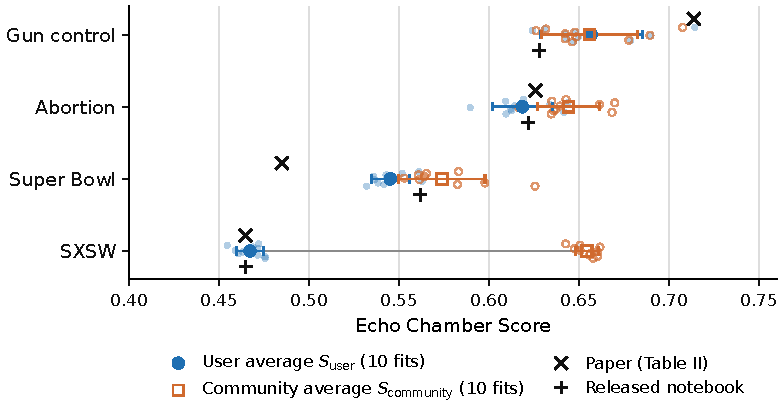
\includegraphics[width=\linewidth]{figure_averaging.pdf}
\caption{Paired reproduction at Louvain seed $42$. For each topic, the ten per-fit $S_{\mathrm{user}}$ values (filled circles) and $S_{\mathrm{community}}$ values (open squares) share the same ten fitted representations; their means are shown with standard-deviation bars. The paper's Table~II value ($\times$) and the notebook's stored value ($+$) are drawn above and below each row for comparison. SXSW is the one row whose user-average mean overlaps the paper's value; its community-average mean sits $0.19$ away.}
\label{fig:averaging}
\end{figure}

The SXSW partition at Louvain seed $42$ contains five non-singleton communities of sizes $1{,}568$, $712$, $85$, $54$, and $17$. Under $S_{\mathrm{user}}$ the largest contributes $64.4\%$ of the weight and the three smallest together contribute less than $7\%$. Under $S_{\mathrm{community}}$ each contributes $20\%$. The three smallest communities have the highest per-community mean scores across the ten fits (around $0.80$--$0.86$), while the largest two have means around $0.40$--$0.48$. The identity $S_{\mathrm{community}}-S_{\mathrm{user}}=\sum_k(1/K-n_k/n)\bar s_k$ in Section~\ref{sec:score} then gives $+0.19$. The three other topics have either two Louvain communities of roughly comparable size (gun control, abortion) or a single dominant community plus small residues with low scores (Super Bowl), so their size-weighted and equal-weighted means stay close.

\subsection{Cross-topic contrast}

The original paper's polarising-minus-non-polarising contrast, $\tfrac{1}{2}(0.714+0.626)-\tfrac{1}{2}(0.485+0.465)$, is $+0.195$. The notebook-stored values give $+0.112$. Our reproduction, evaluated at the reference partition across ten fits, gives $+0.131$ under $S_{\mathrm{user}}$ and $+0.036$ under $S_{\mathrm{community}}$. The sign is positive under both rules; the magnitude under community averaging is roughly a quarter of the user-average magnitude.

Evaluated across all $100$ seed pairs of the crossed design, $10$ pairs are undefined (one Louvain seed on abortion produces a single-community partition). Of the $90$ defined pairs, $S_{\mathrm{user}}$ gives a positive contrast at every pair; $S_{\mathrm{community}}$ reverses sign at $22$. The $22$ reversals come from partitions in which Super Bowl's dominant community shifts in membership and its community mean rises relative to SXSW's small-community means; the reversals are concentrated on three Louvain seeds. A sensitivity sweep over the Louvain resolution hyperparameter is left open; we do not claim the reported fractions generalise beyond resolution $0.05$.

\subsection{Variation decomposition}

Within the $10\times 10$ crossed grid, the balanced-design decomposition attributes a share of the observed squared variation to fitting-seed effects, partition-seed effects, and their interaction. On gun control and abortion partition choice accounts for $0\%$ of the user-score variation (both have two Louvain communities at every seed we tested); on Super Bowl partition choice accounts for $89.0\%$, and on SXSW for $91.8\%$. The complement is split between fitting and interaction. The finite-design decomposition applies to this seed grid and is not an inferential estimate over social populations.

\subsection{Structural response}
\label{sec:structural}

Two rewiring operations change the graph while the seed-$42$ partition is held fixed. The \emph{closure-targeted} rewire uses double-edge swaps that preserve every user's degree and the number of neighbours each user has in every community of that partition. A swap is accepted only if it reduces the triangle count without introducing a duplicate edge or self-loop. The \emph{mixing} rewire preserves only per-user degree and permits community connections to change; it performs ten accepted swaps per original non-loop edge. Each condition draws five graph realisations and three fits per realisation. The encoder is retrained on every graph.

On every graph the closure-targeted rewire reaches zero or a handful of triangles. On every graph the mixing rewire increases the cross-community edge fraction. The mean within-seed delta in $S_{\mathrm{user}}$ for mixing is $-0.155$, $-0.120$, $-0.079$, $-0.037$ on gun control, abortion, Super Bowl, SXSW; all twenty draws decrease. The mean within-seed delta for the closure-targeted rewire is $+0.007$, $-0.003$, $+0.013$, $+0.053$; magnitudes are small, signs are mixed across topics. The retrained ECS responds to cross-community mixing under these conditions and does not respond to triangle removal that preserves community-neighbour counts. The result is scoped to these graphs and this partition.

\section{Discussion of residuals}
\label{sec:residuals}

Three differences remain between the reported, stored, and new values.

\subsection{Paper vs notebook}

The paper's Table~II reports $0.714$, $0.626$, $0.485$, $0.465$. The notebook's stored outputs on the same release are $0.628$, $0.622$, $0.562$, $0.465$. Only SXSW matches. We do not know which execution produced the paper's table. Candidates include an earlier release, a different cached feature file, or hand-tabulation from intermediate values. The paper's gun-control per-community scores ($0.739$ and $0.676$) and sizes ($3{,}984$ and $2{,}582$) are consistent with $S_{\mathrm{user}}$ under rounded inputs, but the reported graph score of $0.714$ is higher than the notebook-stored $0.628$ on the same topic. The two numbers cannot be the same execution. We flag this as an unresolved discrepancy rather than attribute it.

\subsection{New executions vs notebook on Super Bowl}

Our ten-fit user-average mean on Super Bowl is $0.545$, with a range of $0.526$ to $0.566$. The notebook-stored value is $0.562$, at the high end of our range but inside it. The notebook's cached SBERT features may differ from our regenerated ones. A diagnostic run that substitutes the cached file shifts the Super Bowl mean to $0.558$, inside one standard deviation of the stored value. On the other three topics the shift is below $0.005$. The residual Super Bowl discrepancy is therefore in the feature cache and resolves under feature-cache substitution.

\subsection{Encoder width}

The notebook requests widths $20/10$; the function defaults to $100/50$. Across five matched fitting seeds, running at defaults instead of the notebook settings changes $S_{\mathrm{user}}$ by $-0.036$ on gun control, $-0.028$ on abortion, $-0.009$ on Super Bowl, and $+0.012$ on SXSW. The width control does not explain the paper-notebook gap on gun control (opposite sign to the gap), and we do not treat it as the mechanism behind the paper's historical table.

\section{Downstream reporting}

A systematic survey of how downstream work reports ECS values is outside the scope of this reproduction. The recommendation in Section~\ref{sec:conclusion} is motivated by the definitional ambiguity we document, not by a measured prevalence of unspecified reporting. Counting the citing papers that report an ECS value and checking whether each identifies its averaging rule is a useful follow-up; we list it as an open task in the companion repository.

\section{Communication with the original authors}

A draft of this reproduction, including the two-aggregation observation and the residual discrepancies, was sent to the original paper's corresponding author in advance of submission. Any correspondence received before the editorial deadline will be reflected in the final version of this article.

\section{Conclusion}
\label{sec:conclusion}

The reproduction of EchoGAE's SXSW value succeeds under the released code's averaging rule ($S_{\mathrm{user}}$) to within one standard deviation across ten fitting seeds. The three other topics are within $0.07$ of the paper's table under the same rule, and the published cross-topic contrast $(+0.195)$ is recovered in direction $(+0.131)$ if not in magnitude. Classification: Rp.

The reproduction also finds a definitional ambiguity: the paper's Equation~4 and the released notebook compute different quantities under the same name. The difference is small on three topics and large on SXSW, where it reverses the sign of the cross-topic contrast on a fraction of the seed grid. An ECS value cited in subsequent work should name its averaging rule.

\section*{Code and data availability}

Source code, pinned upstream commit, seed-parameterisation patch, regenerated feature manifests, environment lock, and per-topic result files are available at \url{https://github.com/aalok-thakkar/echogae}. A Zenodo mirror will be archived on acceptance for a citable DOI.

